\section{Entwicklung von Performancetests}

Performancetests sind eine nicht-funktionale Art von Tests, die
durchgeführt werden, um die Leistung einer Anwendung zu bestimmen.
Die Tests werden anhand von Metriken wie Geschwindigkeit, Stabilität
und Skalierbarkeit durchgeführt. Die Leistung einer Anwendung zu testen,
ist eine recht umfangreiche und für jede Anwendung spezifische Aufgabe.
Tester müssen die wichtigsten Leistungsindikatoren der Anwendung bestimmen
und eine Reihe von Tests entwerfen. Der Zugang zu diesem Bereich des
Testens wurde jedoch durch das Aufkommen von automatischen Werkzeuge für
Anfänger stark vereinfacht.  Es gibt mehrere kostenpflichtige und kostenlose
Tools, die alle ihre eigenen Vor- und Nachteile haben. In diesem Kapitel
werden keine Vergleiche zwischen diesen Tools angestellt, aber es gibt
Ressourcen, die diesen Vergleich detailliert durchgeführt haben
(vgl. \cite{perfComp}).  Zu den bekanntesten Performancetests Werkzeuge
gehören WebLoad, LoadNinja , LoadView und Apache JMeter. Apache JMeter
ist das Werkzeug, das zum Testen von jExam verwendet wird.

\subsection{Apache Jmeter}


Nach der offiziellen Dokumentation ist Apache Jmeter eine reine
Open-Source-Software, eine 100 \% reine Java-Anwendung, die von Stefano
Mazzocchi von der Apache Software Foundation entwickelt wurde, um das
Funktionsverhalten zu testen und die Leistung zu messen (vgl \cite{jmeter}). Jmeter kann
verwendet werden, um die Leistung von Webanwendungen oder einer Vielzahl
von Diensten zu analysieren und zu messen. Jmeter wurde ursprünglich zum
Testen von Webanwendungen oder FTP-Anwendungen verwendet. Heutzutage wird
es für funktionale Tests, Datenbankserver-Tests. Apache Jmeter kann
verwendet werden, um die Leistung statischer und dynamischer Ressourcen
sowie dynamischer Webanwendungen zu testen. Es kann verwendet werden, um
eine starke Belastung eines Servers, einer Gruppe von Servern, eines
Netzwerks oder eines Objekts zu simulieren, um dessen Stärke zu testen
oder um die Gesamtleistung unter verschiedenen Lasttypen zu analysieren.
Die wichtigsten Vorteile von Jmeter sind :

\begin{enumerate}

    \item \textbf{Open-Source-Lizenz}: Jmeter ist völlig kostenlos und erlaubt
     Entwicklern die Verwendung des Quellcodes für die Entwicklung.

    \item \textbf{Freundliche GUI}: Jmeter ist extrem einfach zu bedienen und es
    dauert nicht lange, sich damit vertraut zu machen.

    \item \textbf{Plattformunabhängig}: Jmeter ist eine 100\% reine
    Java-Desktop-Anwendung. Daher kann es auf mehreren Plattformen laufen.

    \item \textbf{Vollständiges Multithreading-Framework}: Jmeter ermöglicht die
    gleichzeitige und simultane Abtastung verschiedener Funktionen durch
    eine separate Thread-Gruppe.

    \item \textbf{Visualisierung des Testergebnisses}: Das Testergebnis kann in
    verschiedenen Formaten wie Diagramm, Tabelle, Baum und Protokolldatei
    angezeigt werden.

    \item \textbf{Skalierbarkeit}: Jmeter  unterstützt auch Visualisierungs-Plugins,
    mit denen Tests erweitert werden können.

    \item \textbf{Mehrere Teststrategien}: Jmeter unterstützt viele
    Teststrategien wie Lasttests, verteilte Tests und funktionale Tests.

    \item \textbf{Simulation}: Jmeter kann mehrere Benutzer mit gleichzeitigen Threads
    simulieren und eine hohe Last auf die zu testende Webanwendung erzeugen.

    \item \textbf{Unterstützung mehrerer Protokolle}: Jmeter unterstützt nicht
    nur das Testen von Webanwendungen, sondern bewertet auch die
    Leistung von Datenbankservern. Alle Basisprotokolle wie HTTP, JDBC,
    LDAP, SOAP, JMS und FTP werden von Jmeter unterstützt.

    \item \textbf{Aufzeichnung und Wiedergabe}: Jmeter ermöglicht das Aufeichnen
    von Benutzeraktivität im Browser und hilft dabei sie in einer
    Webanwendung zu simulieren.

    \item \textbf{Skript-Test}: Jmeter kann mit Bean Shell für automatisierte Tests
    integriert werden.

\end{enumerate}

Im Allgemeinen hat Jmeter ein vereinfachtes Funktionsprinzip. Es simuliert
eine Gruppe von Benutzern, die Anfragen an einen Zielserver senden, und
gibt Statistiken zurück, die die Leistung/Funktionalität des Zielservers/der
Zielanwendung in Tabellen und Diagrammen zeigen (siehe \Cref{fig:jmeter-prinzip}).

\begin{figure}[H]
    \centering
    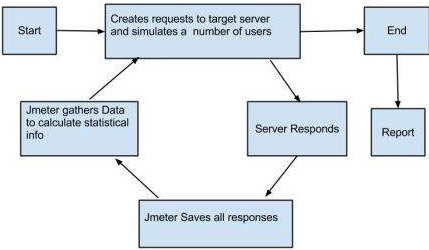
\includegraphics[scale=0.5]{images/jmeter-princip}
    \caption{Funktionsweise von Jmeter} \label{fig:jmeter-prinzip}
\end{figure}

Jmeter wird normalerweise  über seine grafische Benutzeroberfläche
bedient. Es ist  jedoch möglich, Tests mit der grafischen
Benutzeroberfläche zu erstellen und sie in einem Docker-Container auf einer
Anwendung auszuführen. Dieses  Prinzip wurde zum Testen der beiden Versionen
von jExam verwendet und wird  im nächsten Abschnitt vorgestellt.







\subsection{Implementierung der Performancetests}

Die Performancetests, die für beide Versionen von jExam geschrieben wurden,
basieren im Wesentlichen auf den Kriterien in  \autoref{ch:perform}. Die Tests, die
in diesem Kapitel durchgeführt wurden, sind nur eine Demonstration
dessen, was mit JMeter möglich ist. Diese Tests könnten im Laufe der Zeit
weiterentwickelt und verbessert werden, wenn die Kriterien für die Bewertung
der Plattformen spezifischer werden. Sie werden daher als Grundlage für die
Entwicklung zukünftiger Tests dienen. JMeter wird in diesem Fall zum Testen
einer Webanwendung verwendet. Deshalb wird HTTP als Kommunikationsprotokoll
verwendet. Zunächst ist es notwendig, einige Begriffe zu erklären, die im
Folgenden verwendet werden:

\textbf{Thread-Gruppe} : Sie ist eine Gruppe von Threads, die das gleiche
Szenario ausführen. Sie ist das Basiselement für jeden JMeter-Testplan. Es
stehen mehrere Thread-Gruppen zur Verfügung, die konfiguriert werden können,
um zu simulieren, wie die Benutzer mit der Anwendung interagieren, wie die
Last aufrechterhalten wird und über welchen Zeitraum. Jeder Thread führt
den Testplan in seiner Gesamtheit und völlig unabhängig von anderen
Test-Threads aus. Mehrere Threads werden verwendet, um gleichzeitige
Verbindungen zu Ihrer Serveranwendung zu simulieren.

\textbf{Assertions} : Sie sind die Komponente eines Tests, mit der ein
Benutzer bestätigen kann, dass die von JMeter erhaltene Antwort den
erwarteten Kriterien entspricht. Sie stellen sicher, dass der Benutzer sich
einer inkonsistenten oder unerwarteten Antwort der Zielanwendung bewusst
ist. Die Assertions von JMeter sind ein mächtiges Werkzeug, aber ihre
Wirksamkeit hängt sowohl von den ausgewählten Assertionskriterien als auch
von der Genauigkeit der vorherigen Anfrage ab. Die Assertion validiert, dass
die Antwort der Anwendung wie erwartet empfangen wird, aber diese Antwort
beruht in der Regel auf der korrekten Formulierung einer vorherigen Anfrage.


\textbf{Resultslisteners} : Ein Listener ist eine Komponente, die die
Ergebnisse der Proben anzeigt. Die Ergebnisse können in einer Baumstruktur,
in Tabellen oder Diagrammen angezeigt oder einfach in eine Protokolldatei
geschrieben werden.


Für die Integration von Performancetests wurde eine Testsuite entwickelt,
die zwei Tests enthält, die in zwei Thread-Gruppen aufgeteilt sind. Der erste
Test (erste Thread-Gruppe) dient dazu, das Navigieren eines Benutzers auf den
Plattformen zu simulieren und so die Antwortzeiten des Servers zu überwachen.
Auf diese Weise ist es möglich, die beiden Versionen anhand verschiedener
Kriterien zu vergleichen, wie z.B. der schnellsten Antwortzeit. Diese
Thread-Gruppe besteht aus einem einzigen Benutzer und ist in vier Phasen
unterteilt:


\textbf{Login-Phase}: Zunächst führt der Test eine GET-Anfrage an die Login-Seite der
Anwendung durch. Danach führt er auf derselben Seite eine POST-Anfrage durch,
um sich zu registrieren und das Recht zu erhalten, auf gesicherte Seiten
zuzugreifen. Außerdem wurden zwei weitere Assertionen hinzugefügt: die
Duration Assersion, um herauszufinden, ob die Seite in weniger als drei
Sekunden empfangen wird, und die Response Assersion, die sicherstellt,
dass der Test einen korrekten HTTP-Response-Code (200) erhält.


\textbf{Home-Phase}: In diesem Teil führt der Test eine GET-Anfrage an die Home Page
der Anwendung aus. Wenn die Authentifizierung erfolgreich war, sollte der
Test eine HTTP-Response von 200 zurückgeben. Um dies sicherzustellen, wurden
die Assersion Duration (Für die drei Sekunden) und Reponse hinzugefügt.


\textbf{Veranstaltungsphase}: In diesem Teil führt der Test eine GET-Anfrage an die
Veranstaltungsseite aus. Wenn die Authentifizierung erfolgreich war, sollte
der Test eine HTTP-Response 200 zurückgeben. Um dies sicherzustellen, wurden
auch die Assersion Duration und Reponse hinzugefügt.

\textbf{Logout}: In dieser Phase führt der Test eine HTTP-POST-Anfrage aus, um sich
abzumelden, und wie die anderen Phasen verfügt auch diese Phase über die
Assertionen Duration und Response.



Der zweite Test ist viel einfacher. Die Thread-Gruppe besteht aus 200
Benutzern, die in Zeitintervallen von 10 Millisekunden eine GET-Anfrage
an die Home-Seite der Anwendung ausführen. Auf diese Weise können die
Antwortzeiten des Servers bei einer gleichzeitigen Überlastung durch
Anfragen beobachtet werden. Assersion Duration und Response wurden ebenfalls
hinzugefügt.


Nachdem der Tester die Skripte für beide Versionen von jExam geschrieben
und angepasst hat, kann er sie kompilieren und so .jmx-Dateien erzeugen.
Diese Dateien werden dann in Docker Container kopiert, die für die
automatische Ausführung der Tests zuständig sind. Nach der Ausführung der
Tests werden Berichte für \gls{jexam_2009} und \gls{jexam_new} generiert. Der Tester
kann sich diese Berichte ansehen und sie mit den Zielkriterien vergleichen.

\begin{lstlisting}[language=Dockerfile,label={lst:jmeter},caption={JMeter Ausführungsbefehl}]
    command: [ "./wait-for-it.sh", "web:8080/",
"/bin/sh" ,"-c",
"jmeter -f -n -t jExam_New.jmx -l results.csv
-e -o reports/html" ]

# jExam_New.jmx : jExam_new Generierter JMeter-Test
# reports/html : Ordner, der den HTML-Bericht enthalten wird
\end{lstlisting}
